\documentclass[border=6pt]{standalone}
\usepackage{amsmath}
\usepackage{tikz}
\usetikzlibrary{arrows.meta}
\begin{document}
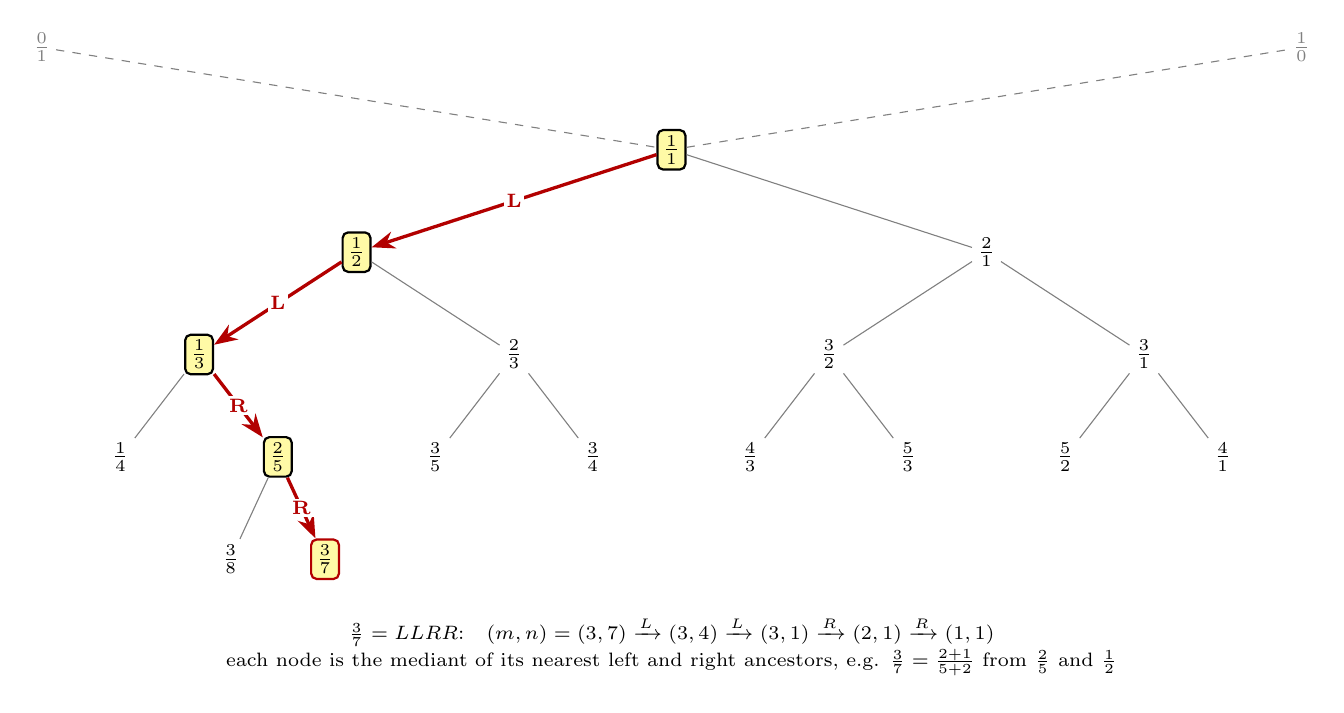
\begin{tikzpicture}[>=Stealth,font=\small,
 s/.style={draw,thick,circle,minimum size=1.1cm,inner sep=0pt,fill=blue!8},
 e/.style={->,thick},
 lab/.style={font=\small,fill=white,inner sep=1.5pt},
 every loop/.style={->,thick,looseness=6}]
\tikzset{f/.style={font=\footnotesize,inner sep=2pt},
 on/.style={f,draw,thick,rounded corners=2pt,fill=yellow!35},
 te/.style={thin,gray},
 pe/.style={->,very thick,red!70!black},
 pl/.style={font=\scriptsize\bfseries,red!70!black,fill=white,inner sep=1pt}}
\node[f,gray] (z) at (-8,1.3) {$\tfrac01$};
\node[f,gray] (inf) at (8,1.3) {$\tfrac10$};
\node[on] (r) at (0,0) {$\tfrac11$};
\node[on] (a) at (-4,-1.3) {$\tfrac12$};  \node[f] (b) at (4,-1.3) {$\tfrac21$};
\node[on] (aa) at (-6,-2.6) {$\tfrac13$}; \node[f] (ab) at (-2,-2.6) {$\tfrac23$};
\node[f] (ba) at (2,-2.6) {$\tfrac32$};   \node[f] (bb) at (6,-2.6) {$\tfrac31$};
\foreach \n/\x/\t in {c1/-7/\tfrac14,c3/-3/\tfrac35,c4/-1/\tfrac34,c5/1/\tfrac43,c6/3/\tfrac53,c7/5/\tfrac52,c8/7/\tfrac41} \node[f] (\n) at (\x,-3.9) {$\t$};
\node[on] (c2) at (-5,-3.9) {$\tfrac25$};
\node[f] (d1) at (-5.6,-5.2) {$\tfrac38$};
\node[on,draw=red!70!black] (d2) at (-4.4,-5.2) {$\tfrac37$};
\foreach \p/\c in {r/b,a/ab,b/ba,b/bb,aa/c1,ab/c3,ab/c4,ba/c5,ba/c6,bb/c7,bb/c8,c2/d1} \draw[te] (\p) -- (\c);
\draw[pe] (r) -- node[pl]{L} (a);
\draw[pe] (a) -- node[pl]{L} (aa);
\draw[pe] (aa) -- node[pl]{R} (c2);
\draw[pe] (c2) -- node[pl]{R} (d2);
\draw[gray,dashed] (z) -- (r) -- (inf);
\node[font=\scriptsize,align=center] at (0,-6.3) {$\tfrac37=LLRR$:\quad $(m,n)=(3,7)\xrightarrow{L}(3,4)\xrightarrow{L}(3,1)\xrightarrow{R}(2,1)\xrightarrow{R}(1,1)$\\each node is the mediant of its nearest left and right ancestors, e.g. $\tfrac37=\tfrac{2+1}{5+2}$ from $\tfrac25$ and $\tfrac12$};
\end{tikzpicture}
\end{document}
